\paragraph{Einleitung}\label{par:stft:intro}
%
Als erstes wollen wir uns mit der Fourier-Analyse von Signalen besch"aftigen.
Hierbei ist das Ziel das Verhalten eines Signals im Frequenzbereich zu charakterisieren.
Wir wollen jedoch in unserer Analyse davon ausgehen, dass wir ein Signal $x[\cdot]$ vorliegen haben, dessen spektrale Eigenschaften \emph{zeitvariant} sind.
Hiermit ist \emph{nicht} gemeint, dass wir davon ausgehen, dass das Signal zeitvariant ist, denn das ist es nat"urlich.
Es geht darum, dass der Anteil der verschiedenen Frequenzen in einem Signal sich mit der Zeit "andert.
Nat"urlich ist hier eine der am einfachsten zug"anglichen Anwendungen die Analyse von Audiosignalen.

Beginnen wir mit einer intuitiven Betrachtung.
Zun"achst wollen wir einen m"oglichst gro"sen Bereich im Frequenzbereich abdecken -- zumindest den f"ur die jeweilige Anwendung relevanten.
Da sich beispielsweise im Audiobereich oft an der menschlichen H"orcharakteristik orientiert wird, die jenseits von \SI{20}{\kilo\hertz} nichts mehr leistet, sind Frequenzen jenseits dieser Grenze nicht mehr relevant.
Das hei"st, dass sinnvollerweise ein Audiosignal mit einer Sample-Rate von \SI{40}{\kilo\hertz} bereits absolut ausreichend aufgenommen wurde.
F"ur andere Anwendungen lassen sich oft "ahnliche Argumente finden, da die meisten physikalischen Systeme eine Tief- oder Bandpasscharakteristik \q{versteckt} haben, und man somit nur sehr selten mit Signalen mit immensen Bandbreiten konfrontiert ist.
Zusammenfassend muss also die Sample-Rate so angepasst werden, dass sie entsprechend unserer Anforderungen ausreicht.

Dar"uber hinaus ist uns aber auch gut daran getan, die Frequenzen, die in dem Signal vorkommen, sehr gut unterscheiden zu k"onnen.
Wir wollen also m"oglichst \emph{genau} wissen, welche einzelnen Frequenzen im Signal vorhanden sind. 
Das hei"st, dass wir f"ur eine tats"achlich im Signal vorhandene Frequenz $F$ aus unserer Analyse eine Frequenz erhalten wollen, die im Intervall $[F-\Delta_1,F+\Delta_1]$ f"ur m"oglichst kleines $\Delta_1 > 0$ liegt.
In diesem Sinne wollen wir also m"oglichst gro"se \emph{Aufl"osung}.
Wenn wir daran denken, dass $\Delta_1 = F_s/N$ gilt, so scheint es zu helfen, dass wir ein Signal m"oglichst lange \q{beobachten} m"ussen, also $N$ sehr gro"s w"ahlen m"ussen.

Doch es gibt noch einen weiteren Aufl"osungsbegriff, der vom ersten strikt zu unterscheiden ist.
Wir wollen au"serdem eine maximale Trennsch"arfe zwischen zwei unterschiedlichen Frequenzen, die gleichzeitig im Signal vorhanden sind, erreichen.
Wir wollen also in unserer Analyse zwei Frequenzen $F_1$ und $F_2$ mit $\Abs{F_1 - F_2} = \Delta_2$ immernoch unterscheiden k"onnen.
Wiederum ist hier das minimale $\Delta_2 > 0$ von Interesse, f"ur das diese Unterscheidbarkeit noch gilt, da dieses ein weiteres Aufl"osungslimit unseres Systems ist.
"Ahnlich wie bei $\Delta_1$ ist auch hier der Beobachtungszeitraum $N$, welchen wir als Grundlage f"ur unsere Analyse verwenden, von Bedeutung. 
Gr"o"ser Zeitr"aume erlauben eine bessere Aufl"osung \emph{zwischen} Frequenzen.

Au"serdem ist es noch oft interessant, dass man einen hohen Dynamikbereich abdecken kann.
Dies meint, dass man Frequenzanteile mit Frequenzen $F_1$ und $F_2$ und Amplituden $A_1$ und $A_2$ noch als zwei wahrnimmt, solange $\log(A_1/A_2) > \Delta_3$. 
Je gr"o"ser das maximale $\Delta_3$ ist, desto besser, da prominente Frequenzanteile nicht weitere weniger stark ausgepr"agte Anteile maskieren.

Schlussendlich haben wir es auch mit zeitvarianten Frequenzanteilen zu tun.
Das hei"st, dass sich zum Zeitpunkt $T_1$ die Zusammensetzung der Frequenzen von denen zum Zeitpunkt $T_2$ unterscheidet.
F"ur $\Abs{T_1 - T_2} > \Delta_4$ wollen wir also erkennen, dass $x(T_1)$ andere spektrale Charakteristik hat als $x(T_2)$ und die f"ur m"oglichst kleine $\Delta_4$.
Diese zeitliche Evolution des Spektrums ist nat"urlich von immenser Bedeutung, weil man m"oglichst genau wissen m"ochte, \emph{wann} sich Frequenzen im Signal ver"andern.
Ideal w"are es also, wenn wir eine Art \q{instantane} Frequenzanalyse durchf"uhren k"onnten, die trennscharf in einem infinitesimalen Intervall die jeweiligen Frequenzanteile aus dem Signal extrahiert.
Doch Schwingungen sind auf inh"arent \emph{ausgedehnte} Effekte.
Ein kleines $\Delta_4$ steht also in direktem Widerspruch zu den Anforderungen an unsere Analyse f"ur, gute (lies: kleine) $\Delta_1$ und $\Delta_2$, da wir dort gesehen haben, dass wir das Signal \emph{lange} beobachten m"ussen.
F"ur diesen Beobachtungszeitraum nehmen wir aber das Signal als \q{konstant} im Frequenzbereich -- also genau kontraproduktiv f"ur ein kleines $\Delta_4$.
%
Wir wollen uns hier lediglich mit der diskreten Version der \gls{stft} befassen, weil wir diese uns als Analysetool von abgetasteten Daten vorstellen, die mit Rate $F_s$ aufgenommen wurden.
Uns liegen also Samples des Signals $x: \R \rightarrow \C$ vor, die wir zum diskreten Signal $x[\cdot]$ abgetastet haben.
%
\paragraph{Definition}
%
Dann definieren wir eine Fensterbreite $W \in \N$ und eine Verz"ogerung $S \in \N$ und bilden die $W$-dimensionalen Vektoren $\bm x_s$ als
\[
\bm x^\ell_n = [x[\ell \cdot S + n]]_{n = 0}^{W-1} \in \C^{W}
\]
und mit diesen eine zweidimensionale Datenstruktur
\[
\bm X = [\bm x^1, \ldots, \bm x^L] \in \C^{W \times L},
\]
welche aus $L$ vielen Teilen von $x[\cdot]$ der L"ange $W$ besteht.
Dann berechnen wir spaltenweise die \gls{dft} auf $\bm X$ und erhalten $\bm X_{\rm stft}$.
%
\paragraph{Interpretation}
%
Im Licht der "Uberlegungen aus \nameref{par:stft:intro} k"onnen wir nun diese Definition interpretieren und noch etwas aufbohren, um bessere Eigenschaften beziehungsweise mehr Information aus der \gls{stft} zu erhalten.
Dabei machen wir uns zunutze, dass eine diskrete \gls{stft} \q{nur} eine blockweise angewandte \gls{dft} ist.
Das hei"st, dass deren Eigenschaften sich ausnutzen lassen, um die \gls{stft} zu beeinflussen.


\clearpage
Zun"achst stellen wir fest, dass wir in einem Block von $\bm{X}_{\rm stft}$ eine Frequenzaufl"osung von $\Delta_1 = F_s / {N W}$, da die Periodendauer eines Blockes im Zeitbereich die L"ange ${WN}/F_s$ hat.
Jetzt k"onnte man auf die Idee kommen, dass man gerne diese Aufl"osung verbessern will.
Eine M"oglichkeit besteht darin die Fensterbreite k"unstlich zu verl"angern.
Eine beliebte Herangehensweise ist an $\bm{X}$ eine bestimmte Anzahl von Nullen anzuh"angen.

Dieses sogenannte \emph{zero-padding} wird in \Cref{py:stft_zp} gezeigt.
Man sieht, dass man bei hinzuf"ugen von $2N$ Nullen an ein Signal der L"ange $N$ eine \emph{Interpolation} der \gls{dft} erreicht.
Diese Technik kann dann \q{blockweise} bei der \gls{stft} angewandt werden, um einen besseren "Uberblick des Spektrums zu bekommen.
Beispielsweise erlaubt dies auch eine genauere Bestimmung des Maximums der \gls{dft}, was der im Signal \q{prominentesten} Frequenz entspricht.
Da wir aber nur Nullen im Zeitbereich anh"angen, entsteht keine neue Information, sondern wir erhalten nur zus"atzliche Zwischenwerte.
F"ur die \gls{stft} hei"st das, dass wir lediglich ein sch"oner aufgel"ostes Bild erhalten, wenn wir zero-padding anwenden.
%
\begin{listing}[ht]
    \noindent
    \begin{minipage}{0.51\textwidth}
        \strut\vspace*{-\baselineskip}\newline
        \inputminted[firstline=4, lastline=20]{python3}{code/stft_zp.py}
    \end{minipage}%
    \begin{minipage}{0.48\textwidth}
        \strut\vspace*{-\baselineskip}\newline
        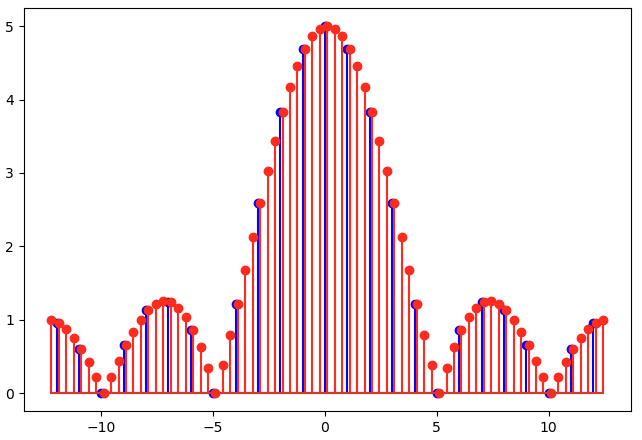
\includegraphics[width=\textwidth]{code/stft_zp.png}
    \end{minipage}
    \codecaption{dsv/code/stft_zp.py}{Zero-padding im Zeitbereich einer $\Rect$-Funktion liefert eine "Uberabtastung der $\Sinc$-Funktion im Frequenzbereich}\label{py:stft_zp}
\end{listing}
%
%
\clearpage
Wir sehen auch noch einen weiteren Effekt von zero-padding, wenn wir ein harmonisches Signal mit der \gls{dft} analysieren.
Die \gls{ft} einer einzelnen Sinusschwingung mit Frequenz $F_0$ entspricht genau zwei komplexen Dirac-St"o"sen bei $\pm F_0$.
Doch was wir im Plot von \Cref{py:stft_harm} sehen ist, dass wir dies im Diskreten nicht reproduzieren k"onnen.
Bei Anwendung der Technik aus \Cref{py:stft_zp} stellt sich heraus, dass wir eher eine Faltung der Dirac-St"o"se bei $\pm F_0$ mit einer $\Sinc$-Funktion sehen.
Deren Auftreten l"asst sich dadurch erkl"aren, dass zero-padding eines Signals der L"ange $N$ auf L"ange $M$ im Zeitbereich der Multiplikation eines Signals mit einem diskreten $\Rect$-Signal entspricht, welches bei $N$ vielen Werten den Wert $1$ annimmt.
Da dessen \gls{dft}, wie in \Cref{py:stft_zp} gezeigt, einem $\Sinc$ entspricht, sehen wir im Frequenzbereich die genannte Faltung.
Wenn wir im Zeitbereich die L"ange des Signals auf $2N$ verl"angern, so multiplizieren wir mit einer \q{breiteren} $\Rect$-Funktion im Zeitbereich und erhalten so einen \q{schmaleren} $\Sinc$ im Frequenzbereich.

F"ur die \gls{stft} hei"st das, genau das, was wir oben schon intuitiv analysiert haben. 
Beobachten wir das Signal in einem l"angeren Block, so k"onnen wir benachbarte Frequenzen besser auseinanderhalten.
Dies gilt jedoch nur, wenn sich diese Zusammensetzung im Frequenzbereich nicht stark "andert, w"ahrend man diese Analyse durchf"uhrt.
%
\begin{listing}[ht]
    \noindent
    \begin{minipage}{0.51\textwidth}
        \strut\vspace*{-\baselineskip}\newline
        \inputminted[firstline=4, lastline=19]{python3}{code/stft_harm.py}
    \end{minipage}%
    \begin{minipage}{0.48\textwidth}
        \strut\vspace*{-\baselineskip}\newline
        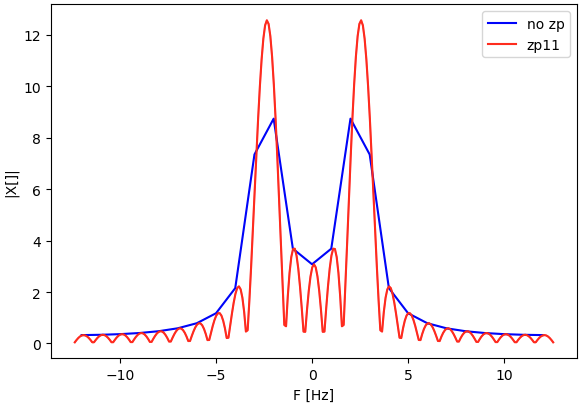
\includegraphics[width=\textwidth]{code/stft_harm.png}

        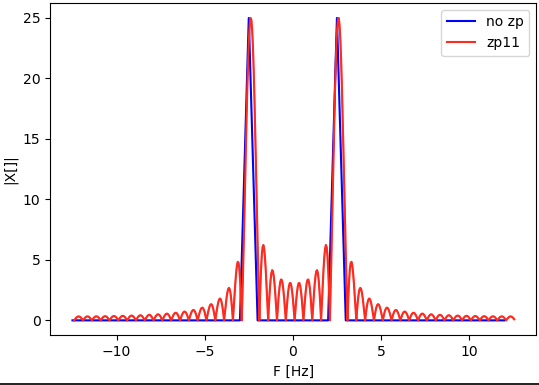
\includegraphics[width=\textwidth]{code/stft_harm_2.png}
    \end{minipage}
    \codecaption{dsv/code/stft_harm.py}{Einfluss der Fensterbreite bei der Analyse von harmonischen Schwingungen}\label{py:stft_harm}
\end{listing}
%
%
\clearpage
Man kann sich diesen Effekt aber auch zunutze machen und somit das Ergebnis der \gls{dft} beeinflussen, indem man das Signal vor der \gls{dft} noch zus"atzlich fenstert, wobei man die Fensterfunktion genau so konzipiert, wie man es gerne h"atte\footnote{\url{https://docs.scipy.org/doc/scipy/reference/signal.windows.html}}.

Wenn wir uns beispielsweise an die Diskussion bez"uglich der m"oglichen Dynamik in einem Signal erinnern, so kann es sein, dass man eher an Dynamik als an Aufl"osung interessiert ist.
In solch einem Fall, kann man beispielsweise auf ein Hann-Fenster\footnote{\url{https://docs.scipy.org/doc/scipy/reference/generated/scipy.signal.windows.hann.html}} zur"uckgreifen und anstatt einem Vektor $\bm x$ transformieren wir mit der \gls{dft} den Vektor $\bm w \odot \bm x$, wobei $\odot$ die punktweise Multiplikation bedeutet.
Dies f"uhrt dazu, dass wir im Frequenzbereich eine Faltung mit der \gls{dft} von $\bm w$ erhalten anstatt einem $\Sinc$.

In \Cref{py:stft_win} sehen wir nun, dass dies erlaubt Frequenzanteile zu finden, die sich ohne explizite Fensterung in den sogenannten Nebenwellen der $\Sinc$-Funktion \q{verstecken}.
Die Nebenwellen der $\Sinc$-Funktion fallen ab gem"a"s
\[
\Abs{\Sinc(x)} \leqslant \frac{1}{x},
\]
wobei andere Fensterfunktionen im Frequenzbereich deutlich schneller abfallen k"onnen.
Wir sehen aber auch, dass sich hier wiederum ein Trade-Off aufzeigt, da die sogenannte Hauptkeule der \gls{dft} von $\bm w$ deutlich breiter ist als die der $\Sinc$-Funktion.
Das hei"st, dass man durch Auswahl der Fensterfunktion zwischen Aufl"osung im Sinne von $\Delta_{1,2}$ und Dynamikbereich w"ahlen kann, beziehungsweise \emph{muss}.
Denn, wie wir gesehen haben, impliziert eine \gls{dft} \emph{immer} eine Multiplikation mit der entsprechenden $\Rect$-Funktion und man kann diese nur gegen eine andere ersetzen, aber nicht vermeiden!
F"ur die \gls{stft} bedeutet dies, dass wir hier  mit derselben Fragestellung konfrontiert sind und entsprechend der gew"unschten Anwendung w"ahlen m"ussen.

\begin{listing}[ht]
    \noindent
    \begin{minipage}{0.51\textwidth}
        \strut\vspace*{-\baselineskip}\newline
        \inputminted[firstline=5, lastline=22]{python3}{code/stft_win.py}
    \end{minipage}%
    \begin{minipage}{0.48\textwidth}
        \strut\vspace*{-\baselineskip}\newline
        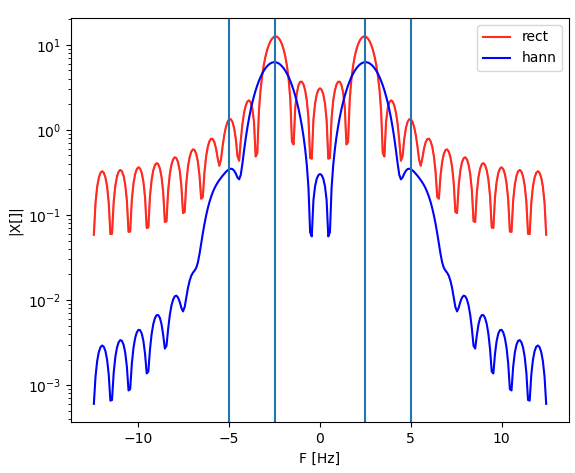
\includegraphics[width=\textwidth]{code/stft_win.png}
    \end{minipage}
    \codecaption{dsv/code/stft_win.py}{Geschickte Fensterung kann den Dynamikbereich erh"ohen}\label{py:stft_win}
\end{listing}
%
%
\clearpage
Als n"achstes wollen wir mit \Cref{py:stft_length} den Punkt machen, dass bei der \gls{stft} direkt Aufl"osung im Frequenzbereich gegen Aufl"osung im Zeitbereich getauscht wird.
Wollen wir genau "Anderungen im Frequenzbereich detektieren, brauchen wir kurze Fenster, opfern daf"ur aber Genauigkeit bei der Loaklisierung der Frequenz.
Andererseits k"onnen wir ein Signal l"anger beobachten und haben sehr gute Aufl"osung im Frequenzbereich, was aber impliziert, dass wir nicht genau sagen k"onnen, \emph{wann} sich Dinge im Frequenzbereich "andern.

\begin{listing}[ht]
    \noindent
    \begin{minipage}{0.51\textwidth}
        \strut\vspace*{-\baselineskip}\newline
        \inputminted[firstline=5, lastline=30]{python3}{code/stft_length.py}
    \end{minipage}%
    \begin{minipage}{0.48\textwidth}
        \strut\vspace*{-\baselineskip}\newline
        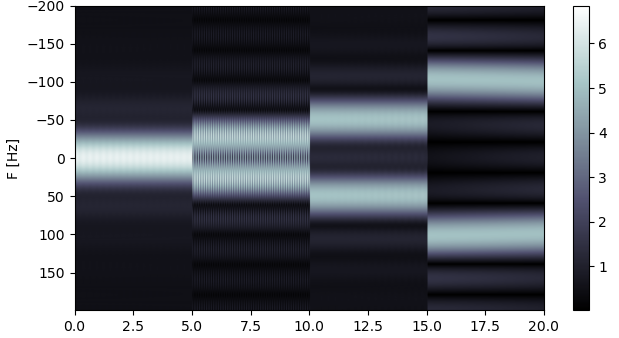
\includegraphics[width=\textwidth]{code/stft_length_1.png}\\
        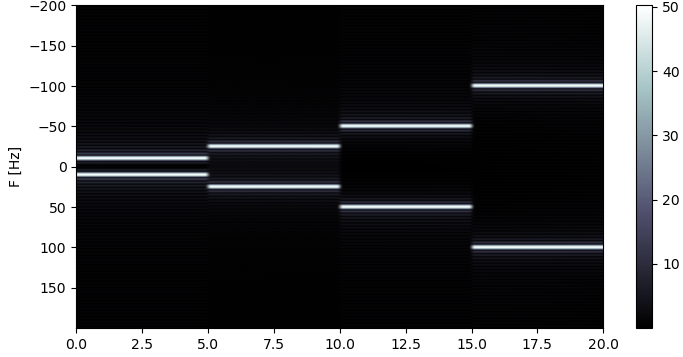
\includegraphics[width=\textwidth]{code/stft_length_2.png}\\
        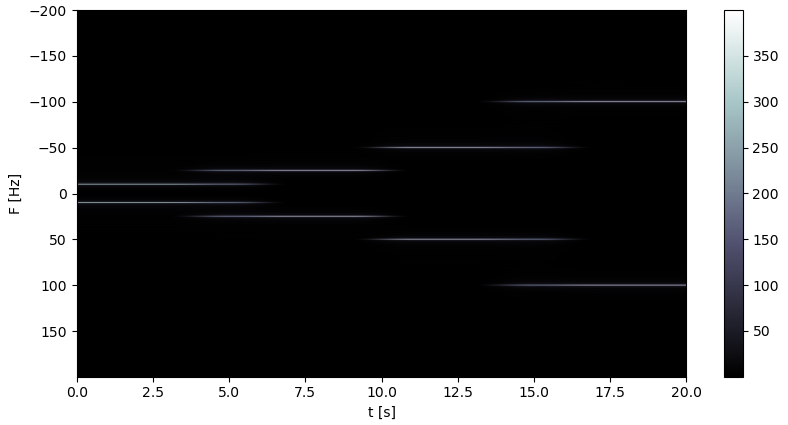
\includegraphics[width=\textwidth]{code/stft_length_3.png}
    \end{minipage}
    \codecaption{dsv/code/stft_length.py}{\acrshort*{stft} f"ur verschiedene Fensterl"angen}\label{py:stft_length}
\end{listing}
%
\clearpage

Als letztes wollen wir ein Beispiel f"ur eine Anwendung der \gls{stft} zeigen. 
In \cref{py:stft_bass} wurde mit einer Bassgitarre eine G-Dur-Tonleiter eingespielt und in entsprechende Bl"ocke zerteilt, die in etwa den einzelnen T"onen entsprechen.
Im Frequenzbereich wurde dann eine \q{peak search} genutzt, um die lokalen Maxima der einzelnen \gls{dft}-Bl"ocke zu finden.
Die ermittelten Frequenzen der einzelnen T"one passen sehr gut zu denen, die man online in Tabellen\footnote{\url{https://mixbutton.com/mixing-articles/music-note-to-frequency-chart/}} finden kann.
\begin{listing}[ht]
    \noindent
    \begin{minipage}{0.51\textwidth}
        \strut\vspace*{-\baselineskip}\newline
        \inputminted[firstline=10, lastline=44]{python3}{code/stft_bass.py}
    \end{minipage}%
    \begin{minipage}{0.48\textwidth}
        \strut\vspace*{-\baselineskip}\newline
        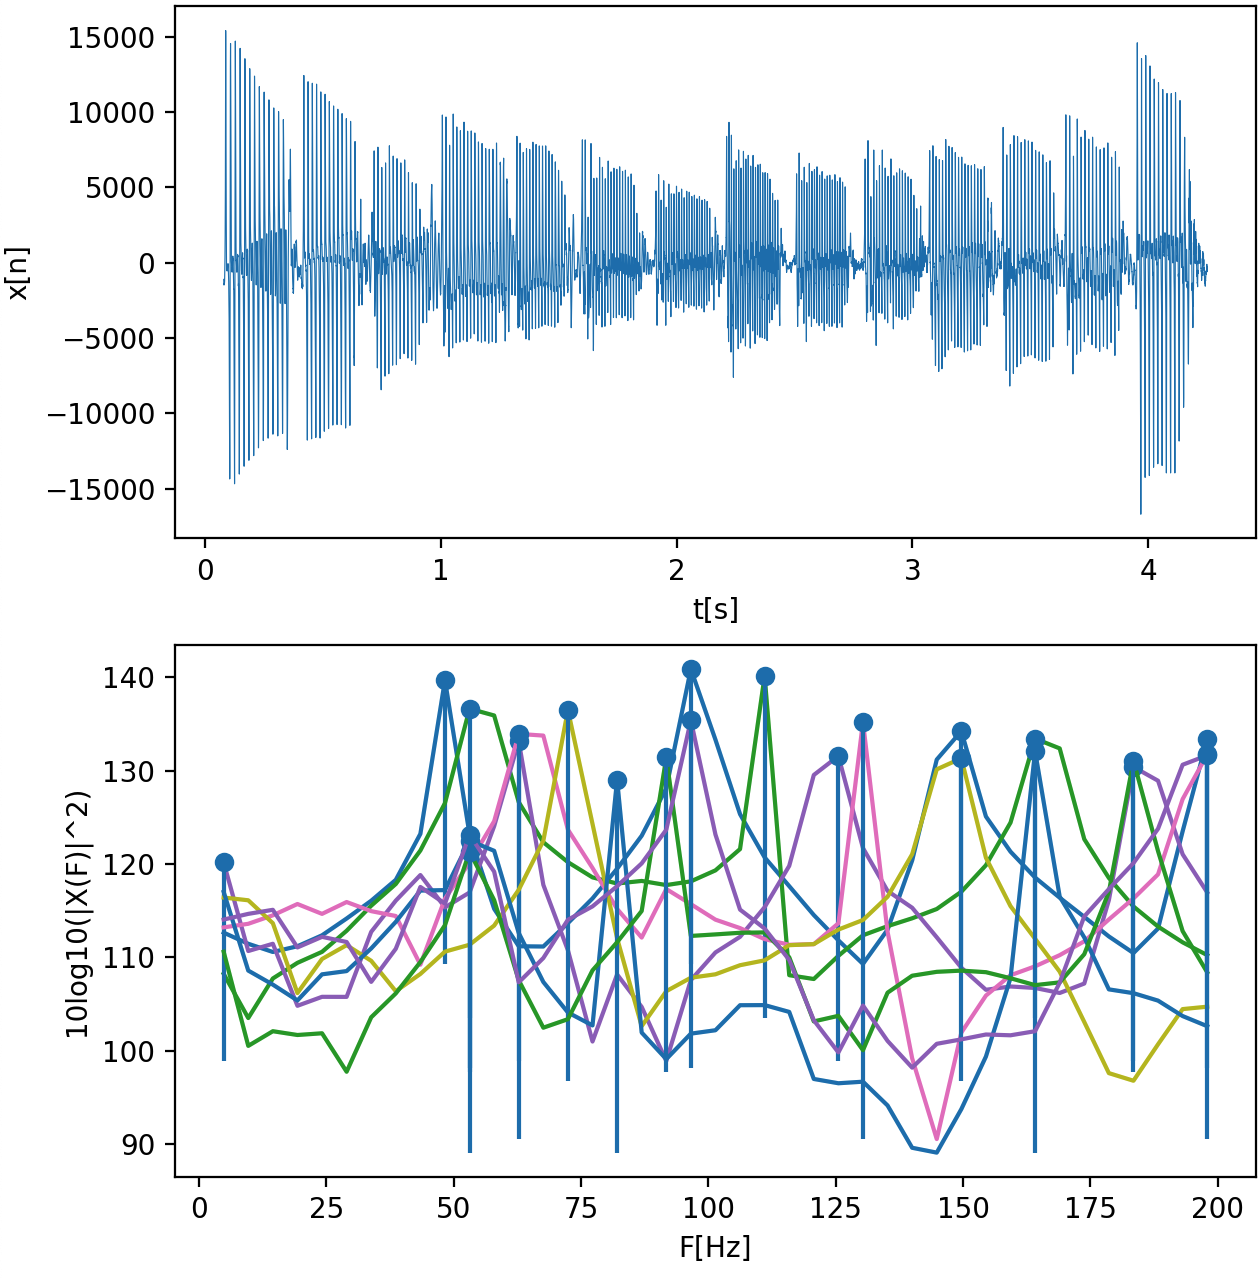
\includegraphics[width=\textwidth]{code/stft_bass.png}\\
    \begin{minted}{python}
    [ 48.2811  96.5622 149.6715 197.9527]
    [ 53.109  111.0466 164.1559]
    [  4.8281  62.7654 125.5309 183.4683]
    [ 62.7654 130.3590 197.9527]
    [ 72.4217 149.6715]
    [ 53.109   82.0779 164.1559]
    [ 53.109   91.7341 183.4683]
    [ 53.109   96.5622 197.95270418]
    \end{minted}
    \end{minipage}
    \codecaption{dsv/code/stft_1.py}{Analyse einer \q{Bassline} mittels \acrshort*{stft}, die eine G-Dur-Tonleiter spielt}\label{py:stft_bass}
\end{listing}

